
\section{Architecture Overview}

\begin{figure}[tbp] \centering
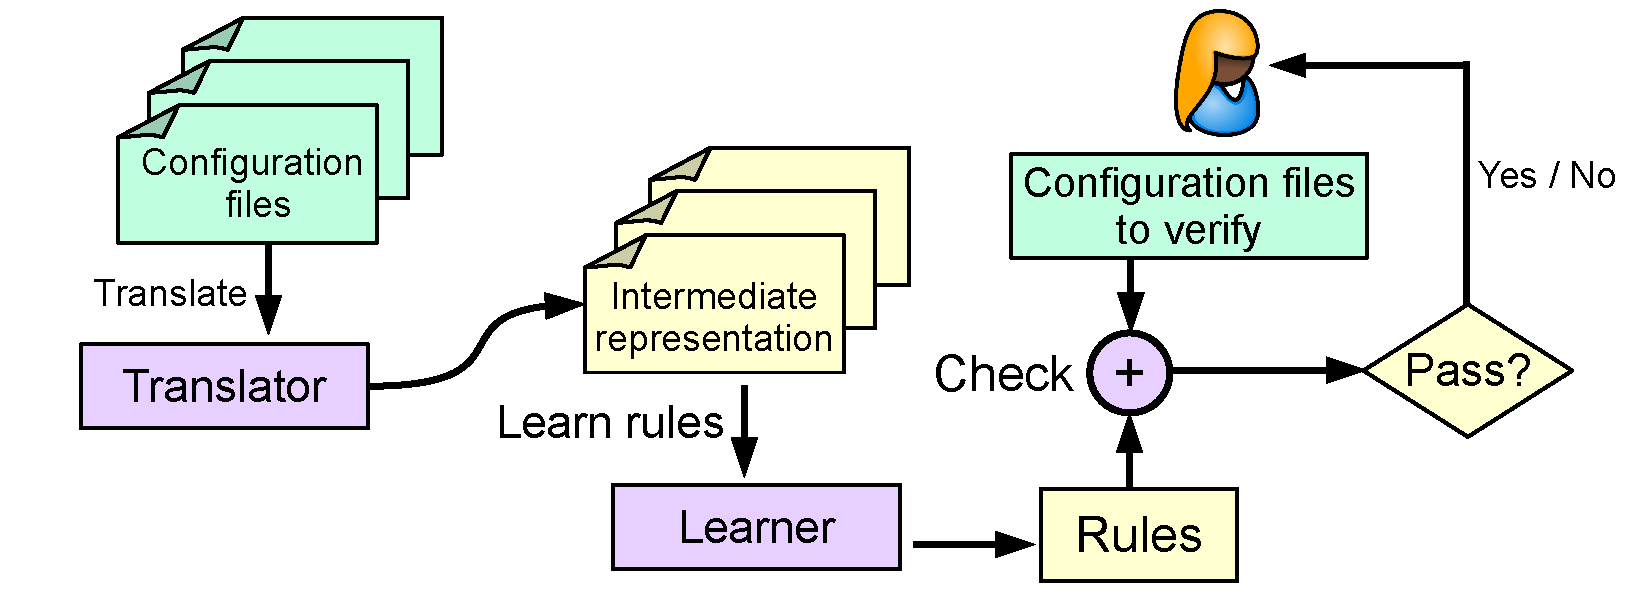
\includegraphics[width=0.78\textwidth]{figs/overview}
\caption{An overview of the \app system architecture}
\label{fig-overview}
\end{figure}




A rule R is added to the set of all rules,
  if $\exists$ learning file f s.t. R(f) is non vacuously true
That rule R is then removed from the set of all rules,
  if $\exists$ learning file f st R(f) is false.

This is accomplished in two passes.
First we collect all possible rules for every file.
Then we merge the all the rules to create our final set.
This conviently gives rise to an embarresingly parallel situation, which Haskell allows us to easily take advantage of by
  using the parallel mapping library parmap.

\begin{lstlisting}
  potentialRules = parmap findAllRules learningSet.
  finalRules = foldl1 mergeRules potenialRules
\begin{lstlisting}


Each rule is of the Attribute typeclass, which means a rule must support the following operations:
\begin{lstlisting}
class Attribute r where
  learn :: ConfigFile Common -> [r]
  merge :: [r] -> [r] -> [r] 
  check :: [r] -> ConfigFile Common -> Error
\end{lstlisting} 


\section{Ordering}
\subsection{learn}
  For a single given file, we take very line ordering to be a rule.
\subsection{merge}
  Then when merging these sets of rules, we take the intersection of the rules infered on the individual files.
  Maybe we could also do something like only taking rules that show up multiple times.
\subsection{check}
  To check a file by using a rule set, we simply take all the rules that are releveant to the user's file.
  Rules that are relavent are the ones where both parts of the ordering are present.
  We learn the rule set for the user file, and every rule in the learned set must be present in the user file.
